\section{Results}\label{results}
All results presented in this section are relative to the application layer. We run simulations on a computer with 2GB RAM memory, CPU intel dual core i3, and Ubuntu 18.04.1 LTS operating system. All runs last 101 seconds with the first second used just for network setup (e.g., nodes requesting connections). The simulation was executed 20 times with $95\%$ of confidence interval.
%Using some \textit{api} from Castalia Simulator some results like the total number of control packets exchanged, the total number of measurements packets, how many times a packets was retransmited among many others results can be obtained easily.

\subsection{Use case and simulation parameters}

Remote Monitoring and Independent living for elderly care is one of the use cases of the X73-PHD standard. The sensors and actuators proposed for this use case are: blood pressure, thermometer, glucose meter, pulse oximeter and basic ECG  \cite{b3}. In this work, we have used an hypothetical elderly patient who has cardiac problems, diabetes and hypertension, and needs to be monitored in his home.

Figure~\ref{fig:wbantopology} shows the topology setup used in our simulation. The hub node is placed at the right hip, a sensor node at each wrist, one sensor node at the each ankle, and one sensor on the chest. We used this set to test our proposed features. These nodes' positions have the advantage of experimental measurements of path loss, made for every pair of nodes, as discussed in \cite{b4}.

\begin{figure}[htbp]
\centerline{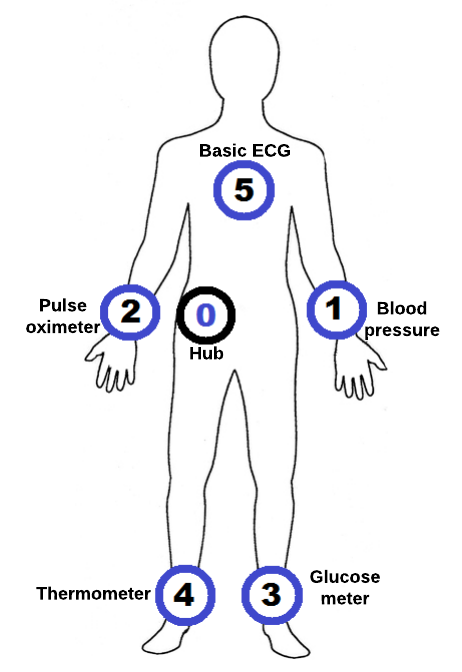
\includegraphics[scale=0.29]{figures/corpoSensoresNomes.png}}
\caption{The simulated network topology.}
\label{fig:wbantopology}
\end{figure}

In this work, we simulate three scenarios. In the first scenario, called \textbf{unconfirmed mode}, agents send measurements with no confirmation by the manager. In the second scenario, called \textbf{retransmission mode}, agents expect an ACK from the manager during three seconds and in case it is not received, the packet is retransmitted up to three times, after that, a new association is made. The third and last one, \textbf{confirmed mode}, agents wait for three seconds the ACK from the manager. If an ACK is not received, the agent has to try to establish a new association to finalize the transmission of the measurement packets. Table \ref{3modes} summarizes the three mentioned modes. 

The MAC layer used is the IEEE 802.15.6 (WBAN) \cite{b5} with path loss map and temporal model for wireless channel supplied by Castalia, and we use a 1024 Kbps physical data rate. The radio used meets with the IEEE 802.15.6 radio proposal \cite{b5} with $-15$dBm as transmission power.
%VINICIUS - Faltou colocar as referências para o padrão do MAC e dizer quantas retransmissões são usadas no retransmission mode% R: Feito
\begin{table}[htbp]
\caption{Operational modes supported by the proposed implementation}
\begin{center}
\begin{tabular}{lllll}
\cline{2-4}
 & \multicolumn{1}{c}{\textbf{\begin{tabular}[c]{@{}c@{}}Unconfirmed\\ mode\end{tabular}}}                      & \multicolumn{1}{c}{\textbf{\begin{tabular}[c]{@{}c@{}}Retransmission\\ mode\end{tabular}}}                                      & \multicolumn{1}{c}{\textbf{\begin{tabular}[c]{@{}c@{}}Confirmed\\ mode\end{tabular}}}                                         &  \\ \cline{2-4}
 & \begin{tabular}[c]{@{}l@{}}The measurements \\ are transmitted\\ with no ACK from\\ the manager\end{tabular} & \begin{tabular}[c]{@{}l@{}}The measurements \\ are retransmitted\\ if an ACK is not\\ received from the\\  manager\end{tabular} & \begin{tabular}[c]{@{}l@{}}If an ACK is not\\ received, try a\\ new association\\ to continue the \\ transmission\end{tabular} &  \\ \cline{2-4}
\end{tabular}
\label{3modes}
\end{center}
\end{table}
The configuration of the nodes is set as follows: the total simulation time is 100 seconds. Node 0 uses the \textit{Manager} application and is the hub. The blood pressure and the pulse oximeter transmit one measurement per second, totalizing 100 measurements to be sent in our simulation. The thermometer sends one read every 2 seconds, then, 50 measurements should be sent. The glucose meter transmits one measurement every 25 seconds, that is, 4 measurements in 100 seconds. In this work, we assume the basic ECG as a device that receives signals of all electrodes deployed in the body, and transmit these signals to the manager. It will transmit 80 millivolt samples per 0.8 seconds, which gives 125 measurement packets in 100 seconds of simulation.

\subsection{Statistical results}

%All the results that will be presented is already implemented in the proposed application and everyone can feel free to customize it. 
%The results available in the application are the total control packets exchanged per node, the measurements packets received by the manager per node, the measurements packets sent by each node, and the total of associations made per agent. 

The first result discussed is the total of successfully measurements delivered to the manager. As described in \cite{b1}, when an agent is working on confirmed mode, it  should send a measurement packet and wait for the ACK during three seconds. 

\begin{figure}[htbp]
\centerline{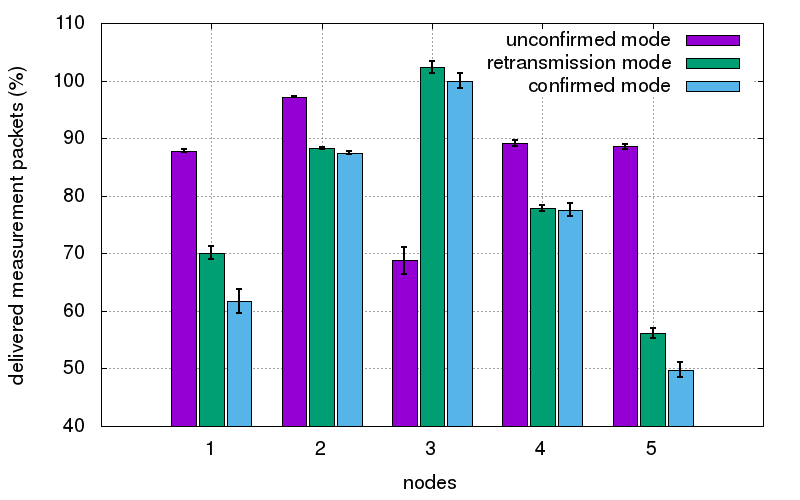
\includegraphics[scale=0.4]{figures/averagemeasurementpacketreceivedpernode.png}}
\caption{Measurement packets successfully delivered per node}
\label{fig:measurementreceivedpernode}
\end{figure}
% VINICIUS - Eu acho que é melhor colocar o gráfico colorido, em percentual e tirar essa legenda de "Which should be transmitted", pq tá poluindo o gráfico desnecessáriamente.

We can see in Fig.~\ref{fig:measurementreceivedpernode} the lack of adaption of the confirmed mode to the scenario, due to lost ACKs, timeouts and disassociation/reassociation processes. The retransmission mode improved the results by reducing the wait time of an association handshake, and retransmitting the messages sooner. The unconfirmed mode delivered almost all packets, although it provides no reliability.
%VINICIUS - Poderia quantificar a melhoria do retransmission em relação ao confirmed%

The overhead of control packets exchanged between a node and the manager is crucial in this scenario, as in the case of a new association due to a non-received ACK. The association procedure involves a maximum of four packets for a new node, and a minimum of two packets, when the agent's attributes are previously known.

The total average of control packets exchanged between each node and the manager per operation mode is depicted in Fig.~\ref{fig:controlpacketsexchanged}. Notice that our retransmission mode saves about $21.5\%$ of control packets when compared to the confirmed mode. The unconfirmed mode as expected is the one that transmits less control packets.

\begin{figure}[htbp]
\centerline{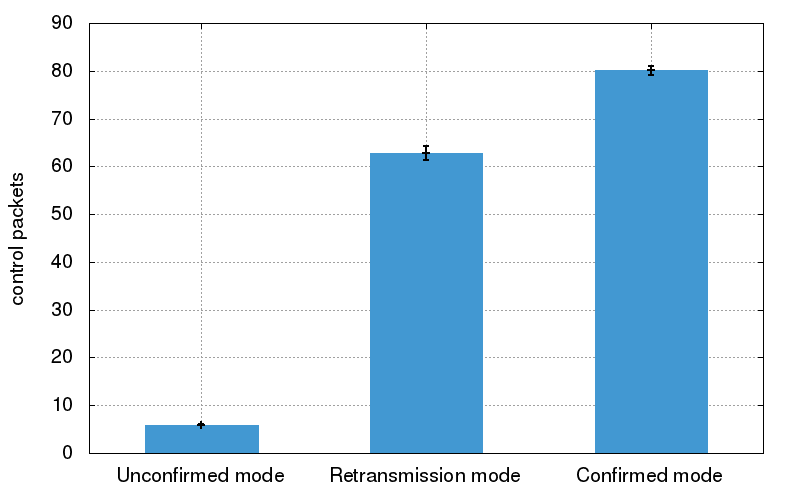
\includegraphics[scale=0.4]{figures/averagecontrolpacketsexchanged.png}}
\caption{The average control packets exchanged of all nodes in each mode}
\label{fig:controlpacketsexchanged}
\end{figure}

The number of associations made per node is extremely high with the confirmed mode, since it tries a new association after every packet lost. Fig.~\ref{fig:associationnumber} shows the average number of associations that each node made in the three operation modes. As expected, the confirmed mode has the highest average of association attempts, while the unconfirmed mode made just one association. The retransmission mode tries a new association after all the attempts to resend a message fail, or if the agent receives an abort message from the manager. This is the reason for the low average of associations in this mode.   

\begin{figure}[htbp]
\centerline{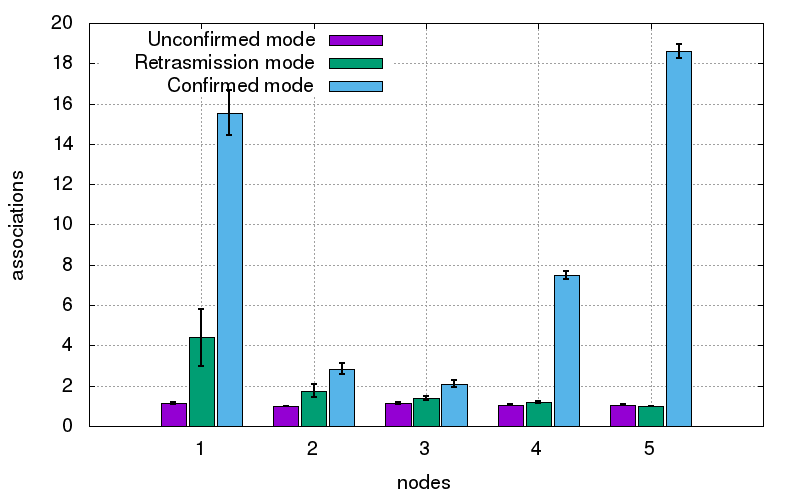
\includegraphics[scale=0.4]{figures/averagetotalassociationsmade.png}}
\caption{The average numbers of association made per node}
\label{fig:associationnumber}
\end{figure}